% prelab2
\documentclass{IEEEtran}
\usepackage{booktabs}
\usepackage{graphicx}
\usepackage{fancyhdr}
\usepackage{framed}
\usepackage{siunitx}
\pagestyle{fancy}
\lhead{}
\chead{}
\rhead{}
\lfoot{}
\cfoot{}
\rfoot{\thepage}
\title{Prelab 2 Amplifiers}
\author{Group 8: Muhan Li \and Man Sun \and Mingxiao An \\ EE233 Circuit Theory}
\IEEEaftertitletext{\centering \vspace{-10pt} \fontsize{11}{11}\textsc{Department of Electrical Engineering, University of Washington, Seattle, WA, 98195} \vspace{10pt}}

\begin{document}
	
	\maketitle
	
	\section{\textbf{Prelab\#1}}
	The typical values of parameters of \textit{LM148} are shown in table[\ref{tab:pl1}], figure[1], and figure[2].
	
	\begin{table}[!htbp]
		\centering
		\caption{The typical values of parameters}
		\begin{tabular}{lcl}
			\toprule
			Parameter & value & \\
			\midrule
			Power supplies & $\pm22\si{V}$ & \\
			Input resistance & $2.5\si{M\Omega}$ & \\
			Slew rate & $0.5\si{V/\mu s}$ & \\
			\bottomrule
		\end{tabular}
		\label{tab:pl1}
	\end{table}
	
	\begin{figure}[!htbp]
		\centering
		\label{fig:101}
		\begin{framed}
			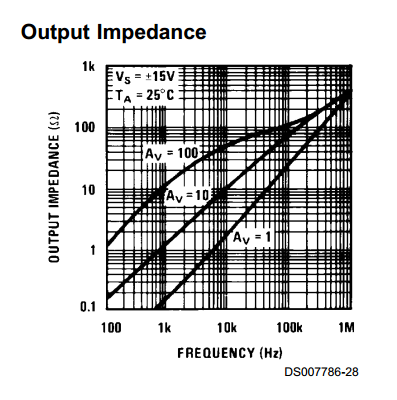
\includegraphics[width=\linewidth]{images/1_1.PNG}
			\caption{Output impedance}
		\end{framed}
	\end{figure}
	
	\begin{figure}[!htbp]
		\centering
		\label{fig:102}
		\begin{framed}
			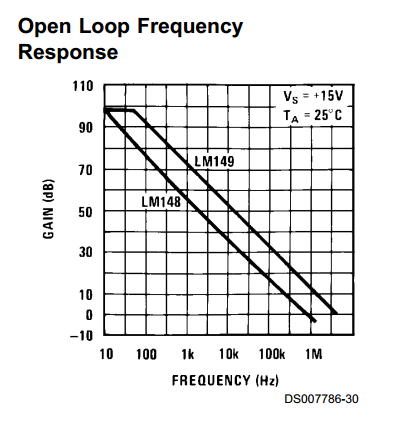
\includegraphics[width=\linewidth]{images/1_2.PNG}
			\caption{Open-loop voltage gain}
		\end{framed}
	\end{figure}
	
	\section{\textbf{Prelab\#2}}
	\begin{equation}
		\mathrm{gain} = \frac{V_{\mathrm{out}}}{V_{\mathrm{in}}} = 1
	\end{equation}
	
	\section{\textbf{Prelab\#3}}
	\subsection{Calculate the time}
	\begin{equation}
		t = \frac{\Delta V}{\mathrm{SlewRate}}
		= \frac{10\si{V}-(-10\si{V})}{0.5\si{V/\mu s}} = 40\si{\mu s}
	\end{equation}
	\subsection{Result comparison}
	The time we read from the datasheet is the gap between the two yellow dots on figure[3]. It is $40\si{ms}$, so we have an error of $0.0\%$. Temperatures, or input resistance, can contribute to error between the theoretical value and actual value.
	\begin{figure}[!htbp]
		\centering
		\begin{framed}
			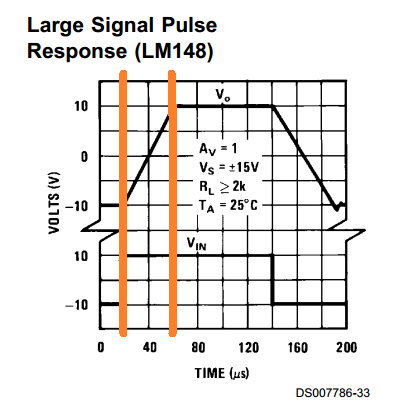
\includegraphics[width=\linewidth]{images/3_1.PNG}
			\caption{Large signal pulse response}
		\end{framed}
	\end{figure}
	
	\section{\textbf{Prelab\#4}}
	\subsection{The expression for the slope of the output voltage}
	\begin{eqnarray}
		\bigg|\frac{\mathrm{d}V_{\mathrm{out}}}{\mathrm{d}t}\bigg| & = & \bigg|\frac{\mathrm{d}V_{\mathrm{in}}}{\mathrm{d}t}\bigg| = \bigg|\frac{\mathrm{d}A\cos(\omega t + \phi)}{\mathrm{d}t}\bigg| \\
		& = & A\omega|\sin(\omega t+\phi)| \\
		& = & 2\pi Af|\sin(2\pi ft+\phi)|
	\end{eqnarray}
	\subsection{The maximum slope of output voltage}
	\begin{equation}
		\bigg|\frac{\mathrm{d}V_{\mathrm{out}}}{\mathrm{d}t}\bigg| = 2\pi Af|\sin(2\pi ft+\phi)| \le 2\pi Af
	\end{equation}
	\subsection{The maximum frequency}
	\begin{eqnarray}
		2\pi Af & \le & SlewRate = 0.5\si{V/\mu s} \\
		f & \le & \frac{0.5\si{V/\mu s}}{2\pi A}
	\end{eqnarray}
	\subsection{The maximum amplitude}
	\begin{eqnarray}
		2\pi Af & \le & SlewRate = 0.5\si{V/\mu s} \\
		A & \le & \frac{0.5\si{V/\mu s}}{2\pi f}
	\end{eqnarray}
	
	\section{\textbf{Prelab\#5}}
	\begin{eqnarray}
		A_{f=100\si{Hz}} & \le & 795.8\si{V} \\
		A_{f=5\si{KHz}} & \le & 15.9\si{V}
	\end{eqnarray}
		
	Since the voltage of audio signals is typically under 2V, which is much lower than $15.9\si{V}$. Thus, we should not be concern about it.
	
	\section{\textbf{Prelab\#6}}
	
	
	\section{\textbf{Prelab\#7}}
	\section{\textbf{Prelab\#8}}
	\section{\textbf{Prelab\#9}}
	\section{\textbf{Prelab\#10}}
	\section{\textbf{Prelab\#11}}
\end{document}

